%! suppress = EscapeHashOutsideCommand
%! Author = Theodore Capinski
%! Date = 4/7/2024

% Preamble
\documentclass[11pt]{article}
\let\oldsection\section
\renewcommand\section{\clearpage\oldsection}
\setcounter{section}{-1}
\counterwithin{figure}{section}

% Packages
\usepackage{amsmath}
\usepackage{hyperref}
\usepackage{graphicx}
\usepackage{tikz}
\usepackage{indentfirst}
\usepackage{calc}
\usepackage{float}
\usepackage{amssymb}

%%%%%%%%%%%%%%%%%%%%%%%%%%%%%%%%%%%%%%%%%%%%%%%%%%%%%%%%%%%%%%%%%%%%%%
% LaTeX Overlay Generator - Annotated Figures v0.0.1
% Created with http://ff.cx/latex-overlay-generator/
%%%%%%%%%%%%%%%%%%%%%%%%%%%%%%%%%%%%%%%%%%%%%%%%%%%%%%%%%%%%%%%%%%%%%%
%\annotatedFigureBoxCustom{bottom-left}{top-right}{label}{label-position}{box-color}{label-color}{border-color}{text-color}
\newcommand*\annotatedFigureBoxCustom[8]{\draw[#5,thick,rounded corners] (#1) rectangle (#2);\node at (#4) [fill=#6,thick,shape=circle,draw=#7,inner sep=2pt,font=\sffamily,text=#8] {\textbf{#3}};}
%\annotatedFigureBox{bottom-left}{top-right}{label}{label-position}
\newcommand*\annotatedFigureBox[4]{\annotatedFigureBoxCustom{#1}{#2}{#3}{#4}{white}{white}{black}{black}}
\newcommand*\annotatedFigureText[4]{\node[draw=none, anchor=south west, text=#2, inner sep=0, text width=#3\linewidth,font=\sffamily] at (#1){#4};}
\newenvironment {annotatedFigure}[1]{\centering\begin{tikzpicture}
                                                   \node[anchor=south west,inner sep=0] (image) at (0,0) { #1};\begin{scope}[x={(image.south east)},y={(image.north west)}]}{\end{scope}\end{tikzpicture}}
%%%%%%%%%%%%%%%%%%%%%%%%%%%%%%%%%%%%%%%%%%%%%%%%%%%%%%%%%%%%%%%%%%%%%%

\newcommand{\todo}[1]{\textcolor{red}{TODO: #1}\PackageWarning{TODO:}{#1!}}

\title{Physics 5BL Lab Report Capstone Project}
\author{T.~Capinski, B. Davis \and A.~Patel}
% Document
\begin{document}
    \maketitle
    \tableofcontents

    \section*{Introduction}\label{sec:introduction}
    \addcontentsline{toc}{section}{Introduction}

    In this report, we will be discussing the results of our capstone project.
    The project was split into three parts.
    The first part was to test different variables in a solenoid to see how they affect the induced current.
    We relied on the formula
    \begin{equation}
        \Epsilon = -N A \frac{d\Phi}{dt}
        \label{eq:emf}
    \end{equation}
    to predict how the voltage would change.
    The second part was to create our own solenoid and test it.
    The third part was to add an iron core to the solenoid to see how it affected the magnetic field.

    We hung a magnet from a spring to create a changing magnetic field.
    This led to an oscillating current being induced in a solenoid.
    We measured the peak induced current for each setup for consistency.

    First, we set up the solenoid with a constant number of turns and one magnet.
    This gave us a baseline for how the solenoid would behave.

    Next, we doubled the number of turns by adding another solenoid in series.
    Based on Equation~\ref{eq:emf}, we expected the peak current to double.
    The result was a voltage $1.92 \times$ as strong as the original setup.
    This agreed with our prediction.

    We then added mass to the spring, which we expected to increase the maximum speed of the magnet, and therefore the rate of change of the magnetic field.
    This led to a voltage $1.02 \times$ as strong as the original setup.
    We realized we had made a mistake in our prediction.
    The mass on the spring does not actually affect the peak current, but rather the damping of the spring.
    By doing the math again, we found that the data was consistent with our new prediction.

    We then tested how the number of magnets affected the peak current.
    We doubled the number of magnets, so based on Equation~\ref{eq:emf}, we expected the peak current to double.
    The result was a voltage $1.78 \times$ as strong as the original setup.


    Finally, we built our own solenoids.
    We did this because we could not vary the radius of the solenoid in the lab.
    We built one with a 3cm radius and one with a 6cm radius.
    We expected the peak current to be $4 \times$ as strong for the 6cm radius solenoid.
    The result was a voltage $4.27 \times$ as strong in the larger solenoid.

    We then added an iron core to the solenoid.
    We expected the peak current to be stronger, but we didn't know by how much.
    The result was a voltage $z \times$ as strong as the original setup.
    We also weren't sure of the exact material of the core, so with this number and some research, we determined it was likely steel.

    Overall, we found how the number of turns, the number of magnets, the mass on the spring, the radius of the solenoid, and the material of the core all affected the peak current.
    Most of our results were consistent with our predictions, but there were some discrepancies.

    \section*{Theory}\label{sec:theory}
    \addcontentsline{toc}{section}{Theory}


Bill's theory, but idk how to attach the picture:
Faraday’s Law states that a changing magnetic flux \(B\) through a single loop will induce an electromotive force (EMF), \(-\frac{d\Phi}{dt}\). Faraday’s Law is applicable to all loops, whether real or imaginary, but it is most readily noticeable in a conducting loop where the induced EMF initiates a current. This current then produces its own magnetic field, adding to the flux within the loop. The presence of a negative sign in the equation is a manifestation of Lenz’s law, which stipulates that the induced EMF current always opposes the change in flux that causes it. 

On this principle, electric motors and generators operate. As we work on building one, let's dive deeper into how it functions.

put a pic here

For our experiment, we used a coil (although we later modified the number of coils, we initially began with just one). We suspended a magnet on a spring and connected it to a dowel. The magnet on the spring was designed to oscillate, causing the magnet to move up and down and creating a changing magnetic field that would induce a current in the coil. The schematic sketch of the setup can be seen above. 

In the final step, we connected the ioLab to the ends of the coils to measure the induced voltage of the setup. We observed a significant increase in voltage when we varied the magnetic strength (i.e., the strength of the magnetic field), the frequency of the oscillations, the number of coils, and particularly the radius of the coil. Now, let's explore our methods and findings in more detail. Follow the experiment procedures outlined below.




    Faraday’s Law states that a changing magnetic flux B through a single loop will induce an electromotive force (EMF), $\epsilon = -\frac{dB}{dt}$.
    Faraday’s Law is applicable to all loops, whether real or imaginary, but it is most readily noticeable in a conducting loop where the induced EMF initiates a current.
    This current then produces its own magnetic field, adding to the flux within the loop.

    The presence of a negative sign in the equation is a manifestation of Lenz’s law, which stipulates that the induced EMF current always opposes the change in flux that causes it.
    On this principle, electric motors and generators operate.
    As we work on building one, let's dive deeper into how it functions.

    \todo{Picture (how generators work). Some theory + formulas.}

    To check that our analysis is correct, we can use agreement test
    \begin{equation}
        |R_{\text{measured}} - R_{\text{expected}}| < 2 \sqrt{\sigma_{R_{\text{measured}}}^2 + \sigma_{R_{\text{expected}}}^2}
        \label{eq:agreement}
    \end{equation}
    where $R_{\text{measured}}$ is the measured ratio, $R_{\text{expected}}$ is the expected ratio, and $\sigma$ is the uncertainty in the measurement.

    \section{Testing different variables}\label{sec:part_1}

    \subsection{Methods}\label{subsec:part_1_methods}

    To test how different variables affect induced current, we set up a solenoid with a constant number of turns.
    We then hung a magnet from a spring and let it oscillate in the solenoid.
    This created a changing magnetic field, which induced a current in the solenoid.
    We measured the peak current for each setup to see how the induced current changed.

    To measure the peak current, we hooked up the solenoid to an IOLab.
    One wire connected to the ground and another connected to A7.
    As the current was induced in the solenoid, it created a voltage across the solenoid.

    Additionally, we placed an IOLab directly above the spring to measure the strength of the magnetic field.
    This we used mostly indirectly in the analysis to compare positions of the magnet between trials, and to verify some data.

    \begin{figure}[H]
        \centering
        \begin{annotatedFigure}
        {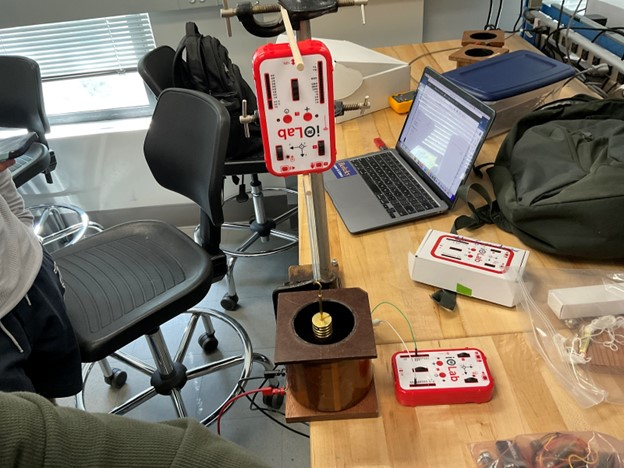
\includegraphics[width=1.0\linewidth]{resources/images/part1a setup}}
            \annotatedFigureBox{0.378,0.6032}{0.577,0.9314}{A}{0.378,0.6032}%bl
            \annotatedFigureBox{0.414,0.0902}{0.613,0.4184}{B}{0.414,0.0902}%bl
            \annotatedFigureBox{0.48,0.2363}{0.546,0.4036}{C}{0.48,0.2363}%bl
            \annotatedFigureBox{0.618,0.1191}{0.8,0.269}{D}{0.618,0.1191}%bl
        \end{annotatedFigure}
        \caption{Our setup for testing different variables in a solenoid. (A) Magnetic Field IOLAb, (B) Solenoid, (C) Magnet, (D) Voltage IOLab.}
        \label{fig:part1a_setup}
    \end{figure}

    Our procedure consisted of the following steps:
    \begin{enumerate}
        \item Set up the solenoid
        \item Hook up the solenoid to an IOLab
        \item Hang the magnet from the spring
        \item Raise the magnet to the maximum height
        \item Release the magnet
        \item Use the IOLabs to measure the peak current and magnetic field strength
        \item Record around 15--30 seconds of data
        \item Repeat steps 3--6 for each variable (number of turns, number of magnets, mass on the spring)
    \end{enumerate}

    Overall, the setup worked well.
    We had some issues with the IOLab not measuring the peak current correctly, but we were able to fix this by adjusting the settings on the IOLab.
    We also had some issues with the magnet remaining attached to the weight set, but we were able to fix this using tape.
    We noticed that the spring would sway side to side as the magnet oscillated, but we determined that this did not significantly affect the results.

    \subsection{Analysis}\label{subsec:part_1_analsysis}

    We first tested how the number of turns affected the peak current.
    We set up the solenoid with a constant number of turns and one magnet.
    We then doubled the number of turns by adding another solenoid in series.
    Based on Equation~\ref{eq:emf}, we expected the peak current to double.

    We want to find how the induced voltage in the first setup compares to the induced voltage in the second setup.

    First, our data is in the form of an oscillating current.
    We want to find the peak current for each setup.
    This can be done by taking all the peaks of the oscillation as our data points.
    Figure \ref{fig:part1_peak_points} shows the current induced in the solenoid for the second setup.
    This was done for each setup, though it will not be shown.

    \begin{figure}[H]
        \centering
        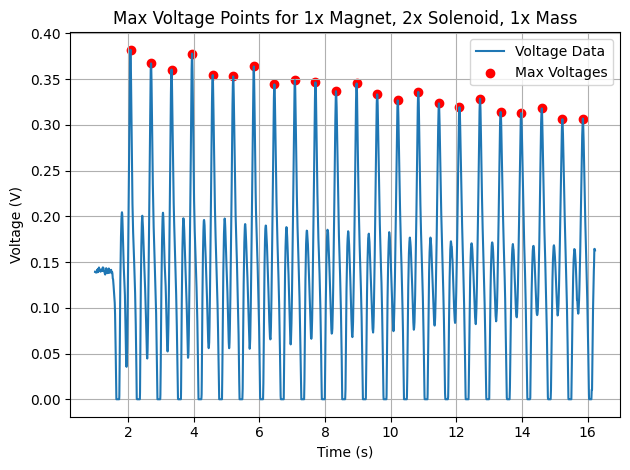
\includegraphics[width=0.8\linewidth]{resources/images/part1 peak points}
        \caption{Graph of the current induced in the solenoid for the second setup, with peaks highlighted.}
        \label{fig:part1_peak_points}
    \end{figure}

    However, before averaging the peaks, we notice the damping.
    This is from the spring, which is not ideal.
    On some trials it is more noticeable than others, but it is always present.
    To be able to compare the two setups, we need to remove the damping.
    Luckily, the damping is linear, so we can fit a line to the damping.
    Then, we can use this line to straighten out the peaks, as if there was no damping.
    While this propagates some error, it is the best we can do.
    The result is shown in Figure \ref{fig:part1a_straightened_points}.

    \begin{figure}[H]
        \centering
        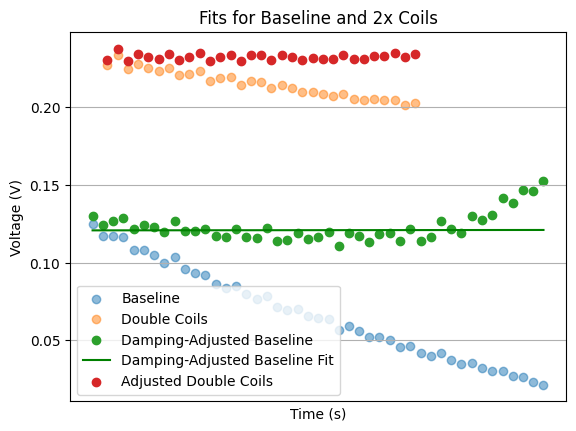
\includegraphics[width=0.8\linewidth]{resources/images/part1a peaks straightened}
        \caption{Graph of the current induced in the solenoid for the first and second setup, with peaks straightened out.}
        \label{fig:part1a_straightened_points}
    \end{figure}

    Now, we can compare the two setups.
    As seen in Figure \ref{fig:part1_straightened_points}, the baseline has been fit to a line.
    This, by design, has a slope of 0.
    It is effectively the average of the baseline peaks.
    The second setup has been straightened out, and the peaks are now easier to compare.

    We can now take each point from the second setup and divide it by the average of the baseline.
    This will give us the ratio of the two setups.
    We can then average these ratios to find the average ratio of the two setups.
    This will give us the factor by which the peak current increased.
    This is shown in Figure \ref{fig:part1a_ratios}.
    Note that this graph also shows that the data points are randomly distributed around the average.
    This implies that the damping was removed correctly, as no pattern is visible.

    \begin{figure}[H]
        \centering
        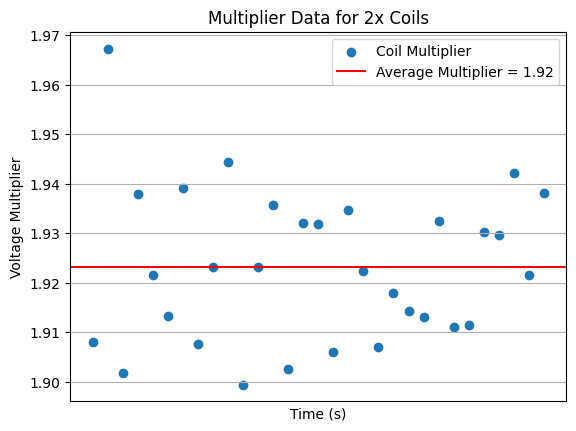
\includegraphics[width=0.8\linewidth]{resources/images/part1a ratios}
        \caption{Graph of the ratio of the two setups.}
        \label{fig:part1a_ratios}
    \end{figure}

    The average ratio of the two setups was 1.92.
    This means that the peak current in the second setup was 1.92 times as strong as the peak current in the first setup.
    This is consistent with our prediction.
    We can use Equation~\ref{eq:agreement} to check if our analysis is correct.

    \begin{align*}
        |1.92 - 2| &< 2 \sqrt{0.20^2 + 0.02^2} \\
        0.08 &< 0.40
    \end{align*}

    We then tested how the mass on the spring affected the peak current.
    We expected the mass to increase the maximum speed of the magnet, and therefore the rate of change of the magnetic field.
    This would lead to a stronger induced current.
    We added mass to the spring and repeated the experiment.
    The result was a voltage 1.02 times as strong as the original setup.
    This can be seen in both Figure \ref{fig:part1b_damping} and Figure \ref{fig:part1b_ratios}.

    \begin{figure}[H]
        \centering
        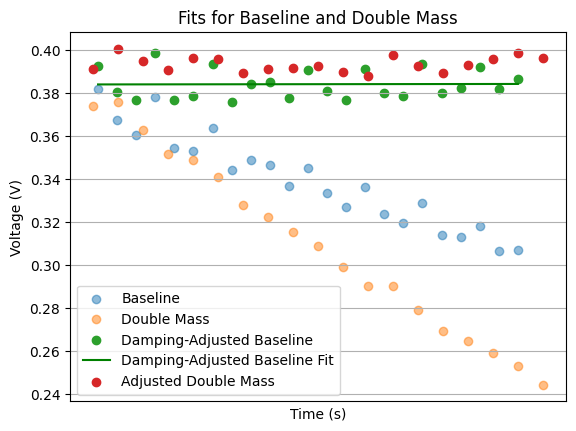
\includegraphics[width=0.8\linewidth]{resources/images/part1b damping}
        \caption{Graph of the current induced in the solenoid for the first and second setup, with damping.}
        \label{fig:part1b_damping}
    \end{figure}

    \begin{figure}[H]
        \centering
        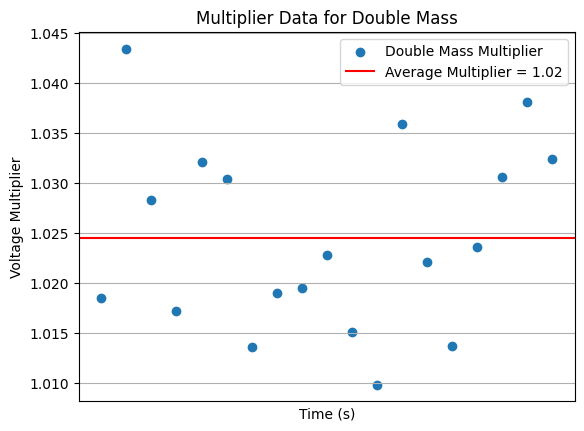
\includegraphics[width=0.8\linewidth]{resources/images/part1b ratios}
        \caption{Graph of the ratio of the two setups. The ratio is only about 1, implying that the mass does not affect the peak current.}
        \label{fig:part1b_ratios}
    \end{figure}

    We realized we had made a mistake in our prediction.
    The mass on the spring does not actually affect the peak current, but rather the damping of the spring.
    By doing the math again, we found that the data was consistent with our new prediction.
    The damping was twice as strong in the second setup, which is consistent with the mass being doubled.
    It went from $4.98 \mu~V/s $ to $9.05 \mu~V/s$.
    This is shown in Figure \ref{fig:part1b_fits}.

    \begin{figure}[H]
        \centering
        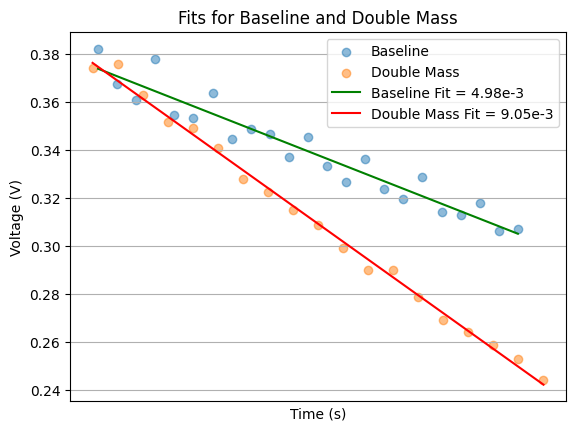
\includegraphics[width=0.8\linewidth]{resources/images/part1b fits}
        \caption{Graph of the damping in the second setup.}
        \label{fig:part1b_fits}
    \end{figure}

    Finally, we tested how the number of magnets affected the peak current.
    We doubled the number of magnets, so based on Equation~\ref{eq:emf}, we expected the peak current to double.
    After repeating the analysis steps, we found that the result was a voltage 1.78 times as strong as the original setup.
    This is shown in both Figure \ref{fig:part1c_damping} and Figure \ref{fig:part1c_ratios}.
    This number is consistent with our prediction.

    We can use Equation~\ref{eq:agreement} to check if our analysis is correct.
    The uncertainty is higher because the damping is higher, but the result is still consistent.

    \begin{align*}
        |1.78 - 2| &< 2 \sqrt{0.29^2 + 0.02^2} \\
        0.22 &< 0.58
    \end{align*}

    \begin{figure}[H]
        \centering
        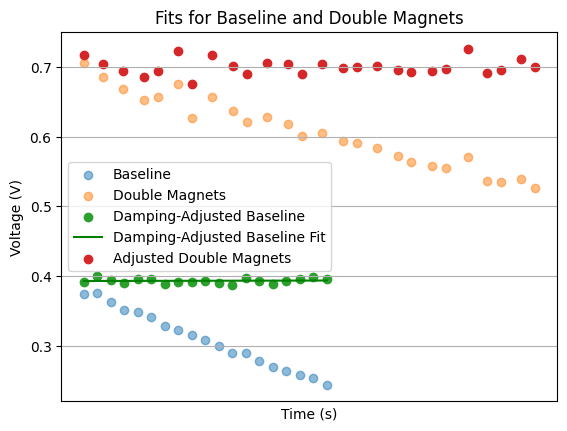
\includegraphics[width=0.8\linewidth]{resources/images/part1c damping}
        \caption{Graph of the current induced in the solenoid for the first and second setup, with damping.}
        \label{fig:part1c_damping}
    \end{figure}

    \begin{figure}[H]
        \centering
        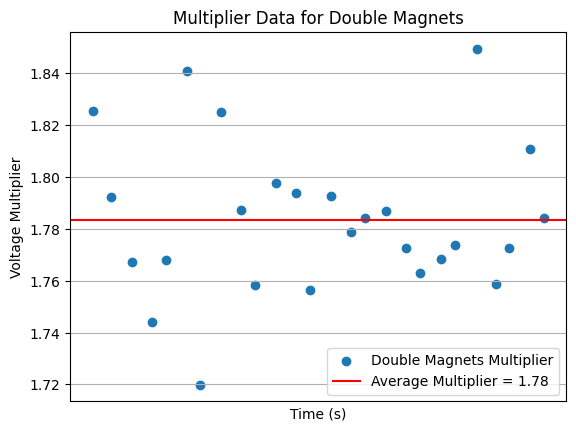
\includegraphics[width=0.8\linewidth]{resources/images/part1c ratios}
        \caption{Graph of the ratio of the two setups.}
        \label{fig:part1c_ratios}
    \end{figure}


    \subsection{Conclusion}\label{subsec:part_1_conclusion}

    In conclusion, we verified how the number of turns, the number of magnets, and the mass on the spring affected the peak current.
    Most of our results were consistent with our predictions, but there were some discrepancies.
    We found that the number of turns and the number of magnets both affected the peak current as expected.
    However, the mass on the spring did not affect the peak current, but rather the damping of the spring.
    This was a mistake in our prediction, but we were able to correct it.
    Agreement tests showed that our analysis was correct for turns and magnets.
    We did not do an agreeement test for the mass change, as the goal of this experiment was to verify how different variables affected the peak current.
    However, we included it in the analysis to show how we corrected our mistake.
    Overall, we were able to verify how different variables affected the peak current in a solenoid.


    \section{Creating our own solenoid}\label{sec:part_2}

    \subsection{Methods}\label{subsec:part_2_methods}

    To create our own solenoids, we found hollow cylinders of different radii.
    For one, we used a Gatorade bottle with a 6cm radius.
    For the other, we used a plastic tube with a 3cm radius.
    We then wrapped wire around the cylinders to create the solenoids.
    Each solenoid had the same number of turns (77).

    We then repeated the experiment from the first part with the new solenoids.
    We measured the peak current for each setup to see how the induced current changed.

    \begin{figure}[H]
        \centering
        \begin{annotatedFigure}
        {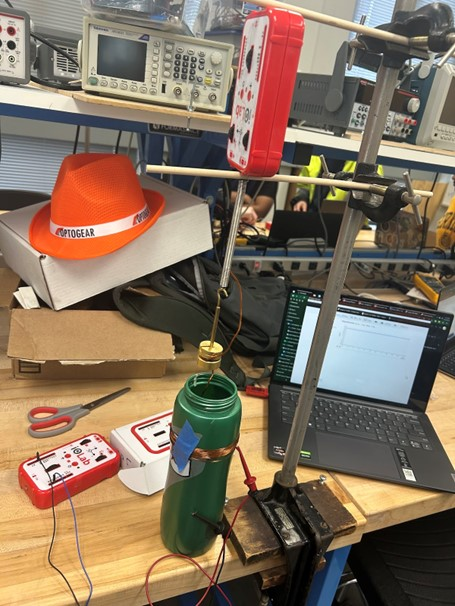
\includegraphics[width=1.0\linewidth]{resources/images/part2a setup}}
            \annotatedFigureBox{0.4819,0.6632}{0.6809,0.9914}{A}{0.4819,0.6632}%bl
            \annotatedFigureBox{0.3421,0.0462}{0.5411,0.3744}{B}{0.3421,0.0462}%bl
            \annotatedFigureBox{0.4214,0.3843}{0.4981,0.5516}{C}{0.4214,0.3843}%bl
            \annotatedFigureBox{0.0453,0.1489}{0.2643,0.3209}{D}{0.0453,0.1489}%bl
        \end{annotatedFigure}
        \caption{Our setup for creating our own solenoids. (A) Magnetic Field IOLAb, (B) Gatorade Solenoid, (C) Magnet and Mass, (D) Voltage IOLab.}
        \label{fig:part2_setup}
    \end{figure}

    \subsection{Analysis}\label{subsec:part_2_analsysis}

    To compare the two solenoids, we repeated the analysis steps from the first part.
    First, we found the peaks of each setup, as shown in Figure \ref{fig:part2_peaks}.
    We then straightened out the peaks to remove the damping.

    \begin{figure}[H]
        \centering
        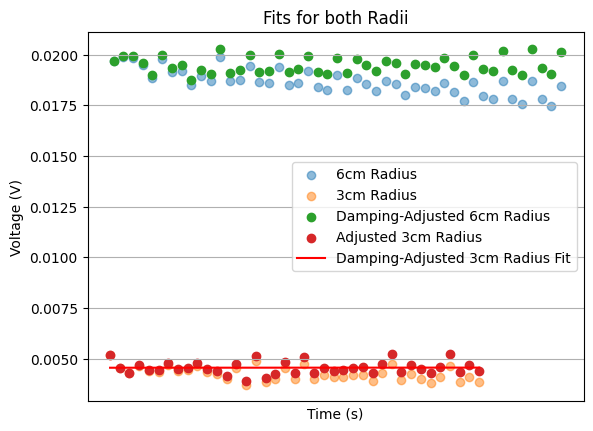
\includegraphics[width=0.8\linewidth]{resources/images/part2 damping}
        \caption{Graph of the current induced in the solenoid for the two setups.}
        \label{fig:part2_peaks}
    \end{figure}

    \begin{figure}[H]
        \centering
        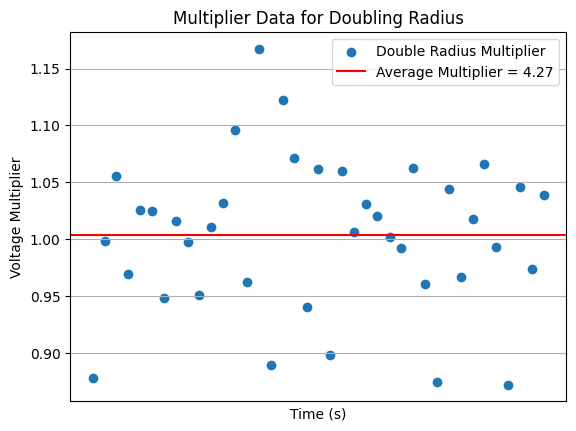
\includegraphics[width=0.65\linewidth]{resources/images/part2 ratios}
        \caption{Graph of the ratio of the two setups.}
        \label{fig:part2_ratios}
    \end{figure}

    We then compared the two setups.
    The larger solenoid was divided by the smaller solenoid to find the ratio of the two setups.
    This was then averaged to find the average ratio of the two setups.
    Additionally, the random distribution of the data points around the average implies that the damping was removed correctly.

    The average ratio of the two setups was 4.27.
    This means that the peak current in the larger solenoid was 4.27 times as strong as the peak current in the smaller solenoid.
    This is consistent with our prediction, as the voltage is proportional to the area of the solenoid.
    We can use Equation~\ref{eq:agreement} to check if our analysis is correct.

    \begin{align*}
        |4.27 - 4| &< 2 \sqrt{0.27^2 + 0.02^2} \\
        0.27 &< 0.56
    \end{align*}

    \subsection{Conclusion}\label{subsec:part_2_conclusion}

    In conclusion, we found that the radius of the solenoid affected the peak current.
    We built one solenoid with a 3cm radius and one with a 6cm radius.
    We found that the peak current in the larger solenoid was 4.27 times as strong as the peak current in the smaller solenoid.
    This was consistent with our prediction.
    Agreement tests showed that our analysis was correct.
    Overall, we were able to verify how the radius of the solenoid affected the peak current.

    \section{Adding a steel core}\label{sec:part_3}
    \subsection{Methods}\label{subsec:part_3_methods}
    In part 3, we changed the self-inductance of the solenoid by adding a steel core to the inside of it. Our base setup can be seen in the following diagram:

    todo add solenoid pic
    caption: Setup for experiment 3 using without steel core. The setup with the steel core is the same, except the steel core is inside the solenoid.

    In this setup, we used 110 grams of mass hanging from the spring with 2 magnets attached to it. 3 premade solenoids were attached, each having 4000 coils. As can be seen in the setup, we used 2 IOLabs - 1 for measuring induced voltage, and the other for measuring spring motion, which did not end up being necessary to use. We then did the following experiments: To perform each experiment, we used the following procedure:

    \begin{enumerate}
        \item Set up the solenoid
        \item Hook up the solenoid to an IOLab
        \item Hang the magnet from the spring
        \item Raise the magnet to the maximum height
        \item Release the magnet
        \item Use the IOLabs to measure the peak current and magnetic field strength
        \item Record around 15--30 seconds of data
    \end{enumerate}

    Since we were unable to get the exact self-inductance of the steel core, as we didn't know exactly what it was or its self-inductance, this section involved more qualitative analysis and comparison between our two trials. Our first trial was the base setup (without the steel core), with the second being the same setup but with the steel core placed inside the solenoid.

    \subsection{Analysis}\label{subsec:part_3_analsysis}
    When we ran this experiment, we got the following raw data:

    todo raw graphs for experiment 3
    caption: Data for experiment 3. The graph titled 'Voltage vs Time for Non-Steel Core Trial' is the data for the trial without the steel core inside. The graph titled 'Voltage vs Time for Steel Core Trial' is the data for the trial with the steel core inside. 

    From this data, we can see that there is a larger damping coefficient for the trial without the steel core. We can see this from the time scale on the x-axis. For the non-steel core trial, the axis has a domain of 0-10 seconds, while the steel core trial ranges from 0-27 seconds. This most likely stems from the fact that the steel core was providing a force on the magnet, which allowed it to maintain a larger amplitude for longer when compared to the trial without the steel core.
    We can also see that the peaks for the trial with the steel core are larger than the non-steel core trial. When we follow a similar procedure as before and account for damping using the peaks of the data, we get the following graphs with adjusted peaks, average voltage lines for these peaks, and their residuals:

    todo put in graphs and residuals
    FIRST: graphs side by side
    caption: Data for experiment 3 with peaks accounted for damping. The graph titled 'Voltage vs Time for Non-Steel Core Trial With Adjusted Peaks' is the data for the trial without the steel core inside. The graph titled 'Voltage vs Time for Steel Core Trial With Adjusted Peaks' is the data for the trial with the steel core inside. 
    SECOND: residuals side by side
    caption: Residuals for average lines for experiment 3 with peaks accounted for damping. The graph titled 'Residuals for Peaks of Non-Steel Core Trial With Adjusted Peaks' is the data for the trial without the steel core inside. The graph titled 'Residuals for Peaks of Steel Core Trial With Adjusted Peaks' for the trial with the steel core inside.

    As we can see from these graphs, we have a larger average voltage for the trial with the steel core inside the solenoid. This value was 0.39 Volts, while the other was 0.35 Volts. However, when we look at the residuals, we can see a pretty clear quadratic pattern in the residuals for the trial with the steel core, while the trial without has no clear pattern. This may also be due to the steel core providing an additional force on the magnet that we have not accounted for during the damping. This tells us that a linear damping fit may not be best for this trial. However, when we do an exponential fitting, we get a very similar graph and the same value for voltage of 0.39 Volts. We can use Equation~\ref{eq:agreement} to check if our values differ enough to conclude a difference in our trials.

    \begin{align*}
        |0.39 - 0.35| &< 2 \sqrt{0.02^2 + 0.02^2} \\
        0.04 &< 0.057
    \end{align*}

    As we can see, the difference in values is inside our error analysis, and we are unable to conclude that adding a steel core increases the self-inductance and thus the induced emf inside a solenoid.

    
    \subsection{Conclusion}\label{subsec:part_3_conclusion}
    In conclusion, we found that adding a steel core to the solenoid did not affect the induced voltage enough to conclude that it increases the self-inductance of the solenoid. This was inconsistent with our prediction because as we can see from equation (todo equation emf = L dI/dt), adding the steel core increases the self-inductance (L) and thus the emf. This may be due to an error inside of our lab. One large unaccounted source of error is the magnetic force from the steel core on the magnet and oscillating masses. While we thought this may have affected the damping of the oscillations (which is decreased), it may have also had an effect on the induced emf in an unpredicted way. We also may have not been precise enough when initializing our magnet's oscillations, as it was hard to keep it exactly the same for each trial. Overall, we were unable to conclude that adding a steel core to the solenoid increased the self-inductance.
    

    \section{Lab Conclusion}\label{sec:lab_conclusion}
    For our capstone project, we worked in the realm of magnetism and electromagnetic induction, exploring various phenomena and conducting experiments to deepen our understanding. We explored the behavior of the induced emf in solenoids when different properties are changed about them.

    In our first experiment, we varied the mass of an oscillating spring with a magnet attached, the number of coils on the solenoid, and the strength of the produced magnetic field from our magnet. By using the IOLabs to measure the induced voltage, we were able to explore how each of these properties affected the induced EMF in the solenoid. For each of these experiments, we were able to confirm our theoretical predictions of the behavior. This experiment not only verified Faraday’s law but also demonstrated the practical application of electromagnetic induction.

    In our second experiment, we created our own solenoids to confirm how changing the radius of a solenoid affects the induced emf. We used a Gatorade bottle and a cylindrical tube to wrap our solenoids around. In this experiment, we were also able to confirm our theoretical predictions of the behavior. By making these solenoids from everyday materials and measuring induced emf as we oscillated a magnet through them, we confirmed Faraday's law and gained practical insights into factors affecting emf strength, reinforcing our understanding of electromagnetic induction's fundamental principles.'

    Lastly, in our third experiment, we increased the self-inductance of our solenoid by adding a steel core inside of it. However, in this experiment, we were unable to confirm our theoretical predictions of the behavior. By incorporating a steel core into our solenoid setup and repeating the experiment, we aimed to explore the effects of increased self-inductance on induced emf. While we were not able to confirm theoretical predictions, we learned how the presence of the steel core influenced the magnetic flux and subsequently, the electromagnetic induction process.


    \appendix
    \section{References}\label{sec:references}

    Lab Manual
\end{document}
